\documentclass{article}

\usepackage{amsmath,amssymb}
\usepackage{geometry}
\usepackage{graphicx}

\geometry{a4paper, margin=2.5cm}

\begin{document}

% ============================================================
\section*{Policy Gradient / REINFORCE}

\subsection*{First, a story}

After DQN we can already beat humans at Atari. But some asked: DQN is fundamentally ``find the best action in each state'' --- that logic works well when actions are discrete, but what about controlling a robotic arm?

Each joint angle of the arm is continuous; the action space is unbounded --- no Q table can be listed, and taking a max over all actions is impossible. The more fundamental issue: DQN learns ``which action is best'' (a Q function); it goes the long way around and never directly tells you ``what the policy should be''.

Is there a more direct route --- \textbf{optimize the policy itself}?

That is the starting point of \textbf{policy gradients}: instead of learning $Q$, parameterize a policy $\pi(a \mid s; \theta)$ and improve it by gradient ascent. REINFORCE is the earliest and most important algorithm on this road.

\textbf{The core question of this chapter}: how do you take a gradient of a policy?

% ============================================================
\section*{From Q Values to Policies}

\subsection*{Two philosophies of RL}

\begin{itemize}
  \item \textbf{Value-based}: first learn $Q(s,a)$, then derive a policy from it (e.g.\ $\varepsilon$-greedy). DQN belongs here.
  \item \textbf{Policy-based}: directly parameterize $\pi_\theta$, maximizing expected total return $J(\theta) = \mathbb{E}_{\tau \sim \pi_\theta}[R(\tau)]$.
\end{itemize}

Advantages of policy gradients:
\begin{itemize}
  \item natural support for continuous actions (output mean and variance, sample from a Gaussian);
  \item the policy is stochastic, with exploration built in --- no extra $\varepsilon$-greedy needed;
  \item a smooth optimization objective with some theoretical guarantees.
\end{itemize}

\subsection*{The question: how to differentiate $J(\theta)$ with respect to $\theta$?}

The expected return is an expectation over trajectories, and the trajectory distribution depends on $\theta$ --- you cannot simply swap the gradient and the expectation.

% ============================================================
\section*{The Log-Derivative Trick}

The key identity:
\[
\nabla_\theta \pi_\theta(a \mid s) = \pi_\theta(a \mid s) \cdot \nabla_\theta \log \pi_\theta(a \mid s)
\]

With this trick the gradient of the distribution moves inside the expectation:
\[
\boxed{\nabla_\theta J(\theta) = \mathbb{E}_{\tau \sim \pi_\theta}\!\left[\sum_{t=0}^{T} \nabla_\theta \log \pi_\theta(a_t \mid s_t) \cdot G_t \right]}
\]

where $G_t = \sum_{k=t}^{T} \gamma^{k-t} r_k$ is the discounted return from step $t$.

\textbf{Intuition}: the meaning is beautiful --- if $G_t$ is large (this path went well), increase $\log \pi(a_t \mid s_t)$ (make this action more likely); if $G_t$ is small, decrease its probability. \textbf{Good behavior gets reinforced; bad behavior gets suppressed}.

% ============================================================
\section*{The REINFORCE Algorithm}

The policy gradient theorem gives the gradient's form, but the expectation cannot be computed exactly --- estimate it by Monte Carlo sampling:

\begin{enumerate}
  \item run one full episode with the current policy $\pi_\theta$, collecting the trajectory $\{(s_t, a_t, r_t)\}$;
  \item compute each step's discounted return $G_t$ (accumulating backwards from the end);
  \item update parameters with the gradient estimate:
\end{enumerate}
\[
\boxed{\theta \leftarrow \theta + \alpha \sum_{t} \nabla_\theta \log \pi_\theta(a_t \mid s_t) \cdot G_t}
\]

This is \textbf{REINFORCE} (Williams, 1992): run a whole episode, then update once, scaling gradients by the return $G_t$ as the ``signal strength'' --- simple and elegant, but with one fatal weakness.

% ============================================================
\section*{High Variance: REINFORCE's Achilles' Heel}

The Monte Carlo estimate is unbiased (the mean over infinitely many samples equals the true expectation) but has enormous variance:
\begin{itemize}
  \item for the same state $s$, the return $G_t$ across episodes can range from 10 to 500;
  \item the update rides entirely on the luck of one trajectory --- a lucky episode gets heavily reinforced, an unlucky one heavily suppressed;
  \item learning curves jitter violently, sometimes spiking then collapsing --- stable convergence is hard.
\end{itemize}

The experiment in Figure~\ref{fig:variance} shows it: five random seeds' raw curves fluctuate wildly, and the smoothed mean stays low --- vanilla REINFORCE cannot reliably solve CartPole-v1 within 500 episodes.

\begin{figure}[!htbp]
  \centering
  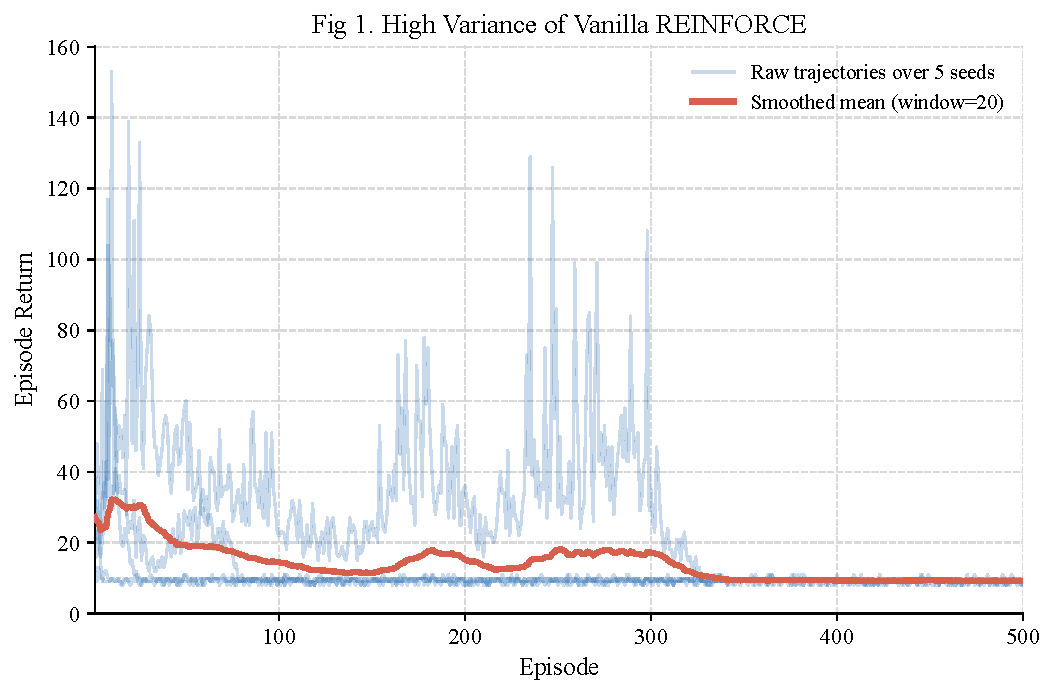
\includegraphics[width=0.95\textwidth]{fig1_reinforce_high_variance.pdf}
  \caption{The high variance of vanilla REINFORCE (CartPole-v1, 5 random seeds). Raw trajectories swing violently --- some episodes spike briefly then fall back --- and the smoothed mean stays at a low level.}
  \label{fig:variance}
\end{figure}

% ============================================================
\section*{Variance Reduction: the Value Baseline}

\subsection*{The core idea}

The root cause: $G_t$ is itself large (CartPole tops out at 500); scaling gradients by it makes step sizes erratic.

The fix: instead of $G_t$, use ``how much better than average'' --- the \textbf{advantage}:
\[
\boxed{A_t = G_t - V(s_t)}
\]

where $V(s_t)$ estimates the expected return in the current state (the baseline). After subtracting the mean, $A_t$ fluctuates around 0 and variance drops sharply.

\subsection*{Why subtracting a baseline does not bias the gradient}

One can show that any function $b(s)$ depending only on the state (not the action) satisfies:
\[
\mathbb{E}_{\tau \sim \pi_\theta}\!\left[\nabla_\theta \log \pi_\theta(a_t \mid s_t) \cdot b(s_t)\right] = 0
\]

So subtracting $V(s_t)$ changes the gradient's \textbf{expectation} not at all, only lowering its \textbf{variance} --- a variance-reduction technique known in statistics as a control variate.

\subsection*{In practice: estimating $V(s)$ with a network}

In practical REINFORCE with baseline:
\begin{itemize}
  \item maintain a \textbf{value network} $V(s;\phi)$ trained by minimizing the squared error $\mathcal{L}(\phi) = \mathbb{E}[(G_t - V(s_t;\phi))^2]$;
  \item the policy gradient becomes $\nabla_\theta \log \pi_\theta(a_t \mid s_t) \cdot A_t$;
  \item the value network's learning rate and capacity must stay restrained --- it should regress the \textbf{expected} return $v^\pi(s)$; if it memorizes the \textbf{realized} $G_t$ of every visited trajectory (overfitting), then on the training data $A_t \approx 0$ and the policy gradient vanishes.
\end{itemize}

\textbf{Relation to Chapter 6}: the ``lower learning rate'' here addresses memorization risk under Monte Carlo regression; Chapter 6's Actor-Critic bootstraps instead, where two-timescale theory requires the critic to learn \textbf{faster} --- different regimes, no contradiction.

The ablation is shown in Figure~\ref{fig:baseline}.

\begin{figure}[!htbp]
  \centering
  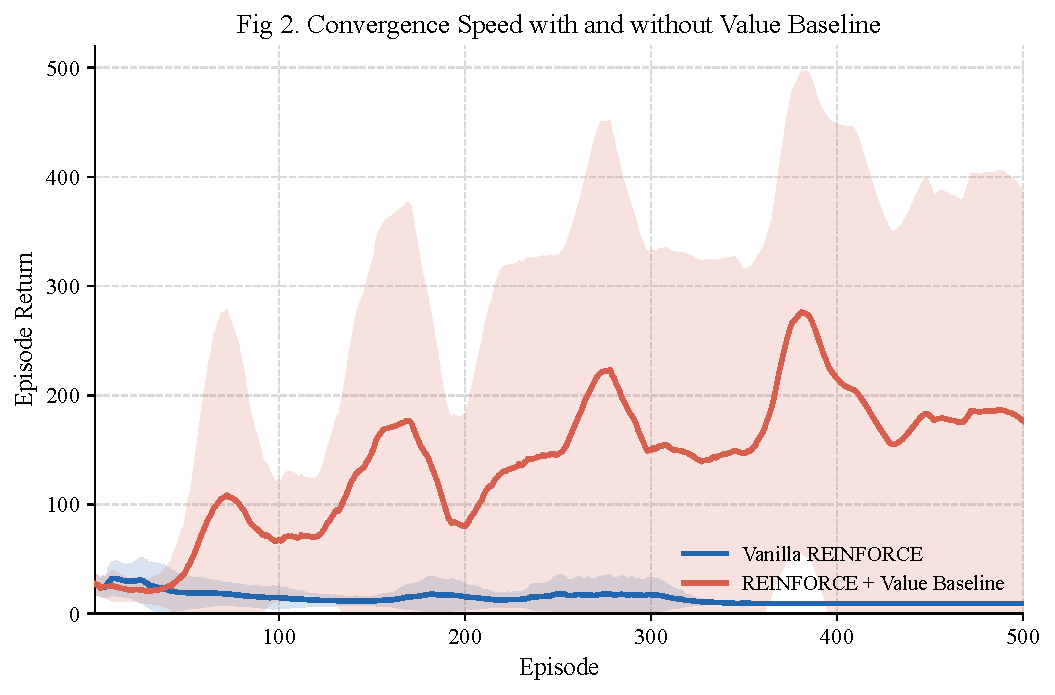
\includegraphics[width=0.88\textwidth]{fig2_convergence_baseline_comparison.pdf}
  \caption{Training with vs.\ without a value baseline (CartPole-v1, 5 random seeds, shading $\pm 1\sigma$). With the baseline, some seeds converge near the maximum within 500 episodes; the overall expected return is markedly higher than vanilla REINFORCE.}
  \label{fig:baseline}
\end{figure}

% ============================================================
\section*{Policy Entropy: from Random to Deterministic}

The \textbf{policy entropy} is:
\[
H(\pi(\cdot \mid s)) = -\sum_a \pi(a \mid s) \log \pi(a \mid s)
\]

For CartPole's two actions, the uniform policy's entropy is at most $\ln 2 \approx 0.693$ nats. Falling entropy means the policy moves from ``mashing randomly'' toward ``committing''.

Figure~\ref{fig:entropy} shows the entropy trajectories of both methods during training:

\begin{figure}[!htbp]
  \centering
  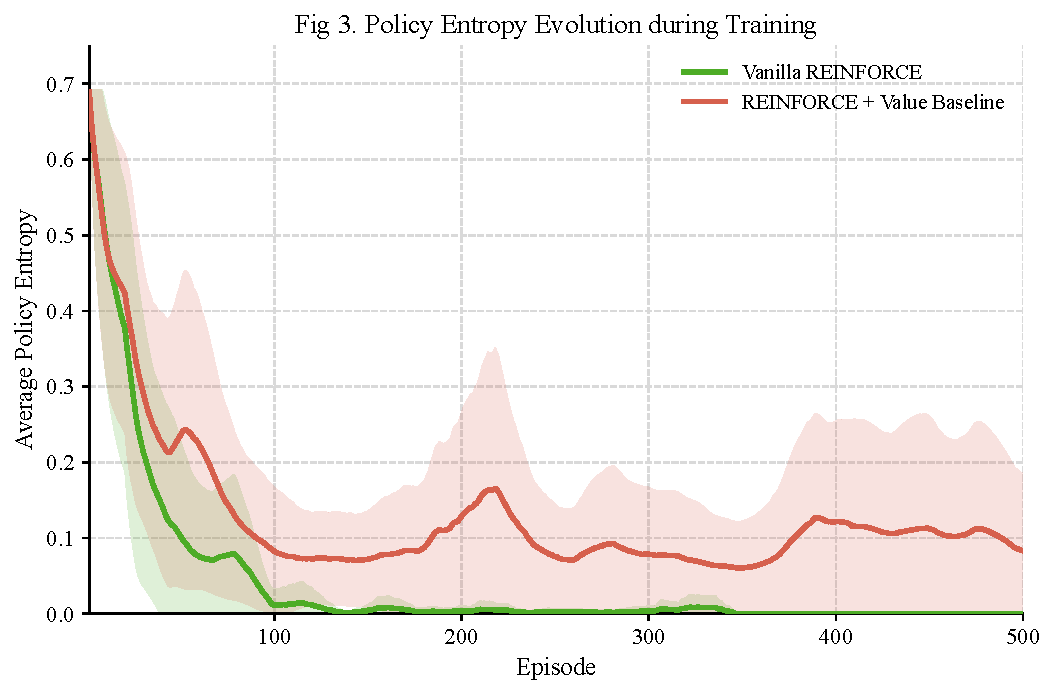
\includegraphics[width=0.88\textwidth]{fig3_policy_entropy_evolution.pdf}
  \caption{Policy entropy during training (CartPole-v1, 5 random seeds, shading $\pm 1\sigma$). Vanilla REINFORCE's entropy collapses to near zero without converging to a good policy --- premature commitment to a bad deterministic policy; the baseline version's entropy declines more gently, exploration survives, and the final policy is better.}
  \label{fig:entropy}
\end{figure}

The contrast reveals an instructive phenomenon: rapidly falling entropy does not mean ``learning well'' --- vanilla REINFORCE's entropy is nearly zero after about 100 episodes while its return stays low (Figure~\ref{fig:variance}). The policy has prematurely committed to a bad deterministic behavior (say, always pushing one direction); with exploration gone, no further improvement is possible. The value baseline provides a steadier learning signal, letting the policy keep exploring and eventually find better behaviors.

% ============================================================
\section*{The Full Algorithm: REINFORCE with Value Baseline}

\begin{enumerate}
  \item \textbf{Initialize}: policy network $\pi(a \mid s;\theta)$, value network $V(s;\phi)$;
  \item \textbf{Each episode}:
    \begin{enumerate}
      \item run a full episode with $\pi_\theta$, collecting $\{(s_t, a_t, r_t)\}_{t=0}^T$;
      \item compute discounted returns backwards: $G_t = \sum_{k=t}^T \gamma^{k-t} r_k$;
      \item update the value network: $\phi \leftarrow \phi - \alpha_V \nabla_\phi \sum_t (G_t - V(s_t;\phi))^2$;
      \item compute advantages: $A_t = G_t - V(s_t;\phi)$ (detached; no gradient flows);
      \item update the policy: $\theta \leftarrow \theta + \alpha_\pi \sum_t \nabla_\theta \log \pi_\theta(a_t \mid s_t) \cdot A_t$.
    \end{enumerate}
\end{enumerate}

\textbf{Hyperparameter notes}:

\begin{center}
\small
\begin{tabular}{l|l}
\textbf{Setting} & \textbf{Reason} \\
\hline
$\alpha_V < \alpha_\pi$ & guard against $V(s)$ overfitting realized returns (memorization drives $A_t \approx 0$) \\[4pt]
no z-scoring of $A_t$ & $V(s)$ already centers the signal; extra normalization can erase it \\[4pt]
clip\_grad\_norm & single-trajectory gradients have huge variance; clipping prevents oversized steps \\
\end{tabular}
\end{center}

% ============================================================
\section*{Where policy gradients sit in the RL landscape}

REINFORCE is the origin of policy-gradient methods:

\begin{enumerate}
  \item \textbf{From values to policies}: Q-learning/DQN optimize $Q$ and derive a policy indirectly; policy gradients optimize $\pi_\theta$ directly --- clearer objective, natural continuous-action support;
  \item \textbf{The price of Monte Carlo}: REINFORCE waits for the whole episode before updating --- low data efficiency, high variance; this motivates the next step;
  \item \textbf{Actor-Critic (A2C/A3C)}: replace REINFORCE's Monte Carlo return $G_t$ with a TD estimate (bootstrapping), updating before the episode ends. Actor (policy) and Critic (value) train together, balancing variance and bias;
  \item \textbf{PPO / TRPO}: add update-magnitude constraints on top of Actor-Critic to keep one update from wrecking the policy; PPO is the most widely used policy-gradient algorithm in industry --- ChatGPT's RLHF training builds on it;
  \item \textbf{The continuous-control mainline}: DDPG, TD3 and SAC extend policy gradients to continuous actions, becoming the standard for robot control.
\end{enumerate}

\subsection*{References}

\begin{enumerate}
  \item Williams, R.\,J.\ (1992). Simple statistical gradient-following algorithms for connectionist reinforcement learning. \textit{Machine Learning}, 8, 229--256.
  \item Sutton, R.\,S.\ \& Barto, A.\,G.\ (2018). \textit{Reinforcement Learning: An Introduction} (2nd ed.). Chapter 13: Policy Gradient Methods.
  \item Schulman, J., et al.\ (2015). Trust Region Policy Optimization. \textit{ICML}.
  \item Schulman, J., et al.\ (2017). Proximal Policy Optimization Algorithms. \textit{arXiv:1707.06347}.
  \item Hands-on RL (Chinese). Chapter 9: policy gradient algorithms.
\end{enumerate}

\end{document}
